%Project Narrative
\documentclass[11pt,letterpaper]{article}
\usepackage[margin=1in]{geometry}
\usepackage[]{natbib}
\bibpunct[; ]{[}{]}{,}{n}{}{;} 
\bibliographystyle{unsrtnat}
\setcitestyle{plain}
\usepackage{color}
\usepackage{graphicx}
\usepackage{url}
\usepackage{multicol}
\usepackage{wrapfig}
\usepackage{amsmath}
\usepackage{amssymb}
\usepackage{caption}
\usepackage{subcaption}
\usepackage[usenames,dvipsnames,svgnames,table]{xcolor}
\usepackage[innercaption]{sidecap} % side captions
\sidecaptionvpos{figure}{c}
\usepackage{parskip}

\begin{document}

\title{\vspace{-5ex}Research Approach: Evolutionary genomics of maize\vspace{-4ex}}
\author{}
\date{}
\maketitle


%Research Approach - not to exceed 1,500 words - of your ongoing and planned research program.
%May include a list of essential references and up to one page of figures.
%Figures and accompanying short legends may be interleaved with the body of the research approach text.
%Figures, legends, and essential references are not included in the 1,500 word limit.

%INTRO 376 words

My research program applies population genomic approaches to investigate how plants evolve.
Agricultural plants provide a particularly excellent system for basic discovery, with their rich history of basic genetic research, ample modern genomic resources, and the opportunity to sample or replicate genotypes across a wide array of environments.
Among crop plants, maize provides perhaps the best opportunity for basic research and discovery.
In addition to its status as the country's most valuable crop, maize is also one of the oldest model organisms, and its rich phenotypic and genetic diversity have enabled a number of basic scientific discoveries, from hybrid vigor \citep{shull1908composition} to the relationship between crossing over and recombination \citep{creighton1931correlation}, meiotic drive \citep{rhoades1942preferential}, and transposable elements \citep{mcclintock1950origin}. 
Maize continues to be an important model in the genomics era \citep{nannas2015genetic}, and the publicly available resources are unparalleled among other crops: genome and whole-genome genotypes number in the tens of thousands, and association mapping studies now approach scales rarely seen outside of biomedical studies \citep[e.g.][]{buckler2009genetic,peiffer2014genetic,Romay2013,Hearne2015}.

Maize is particularly well-suited as a model to study plant evolution.
Domestication and modern breeding can be seen as experimental evolution, and both population genomic \citep{hufford2012comparative} and archaeological data \citep{purugganan2011archaeological} suggest that the rate and magnitude of adaptation in these situations is likely similar to that found in natural populations.
While maize has a large genome compared to many other model plants --- the maize reference is 2.3Gb \citep{schnable2009b73} ---  it is in fact close to the median for most flowering plants \citep{leitch2013genome}, and thus an ideal organism in which to study transposable elements and other structural variation that abound in complex plant genomes.  
Finally, the wild relatives of maize, collectively referred to as teosintes, inhabit a diverse array of environments and include both endangered species and taxa with large, stable, randomly-mating populations \citep{hufford2012teosinte}.
Because all of these species are closely related, we can easily transfer genomic resources developed in maize to these wild taxa as well \citep[e.g.][]{pyhajarvi2013complex,fang2012megabase}.
Though there are numerous efforts in maize to accelerate crop breeding, there are surprisingly few efforts to take advantage of these resources to study maize evolution. 
My group has taken the lead in evolutionary analyses of maize and its relatives; below I describe current and planned research towards understanding plant adaptation and genome evolution.  

\section*{Experimental Evolution} % 406

Plant domestication and modern breeding essentially represent examples of experimentally evolved populations. Studying these populations represents an opportunity to understand not only the genetic basis of evolutionary change (which alleles were selected), but also how the processes of evolution --- particularly the interaction of selection and demographic change --- shape modern genetic and phenotypic diversity.

We have worked to understand the process of selection during domestication, documenting its polygenic nature, the contributions of regulatory variation \citep{hufford2012comparative,swanson2012reshaping}, and the importance of processes such as convergent molecular evolution \citep{wills2013many} and selection on standing genetic variation \citep{wills2013many, studer2011identification, vann2015natural}. 
Our detailed analyses of  inbred lines have revealed little evidence for strong selection during modern maize breeding, instead highlighting the effect of small population sizes in partitioning diversity into distinct populations of increasingly narrow ancestry \citep{van2012historical}.

\begin{figure*}[t]
\centering
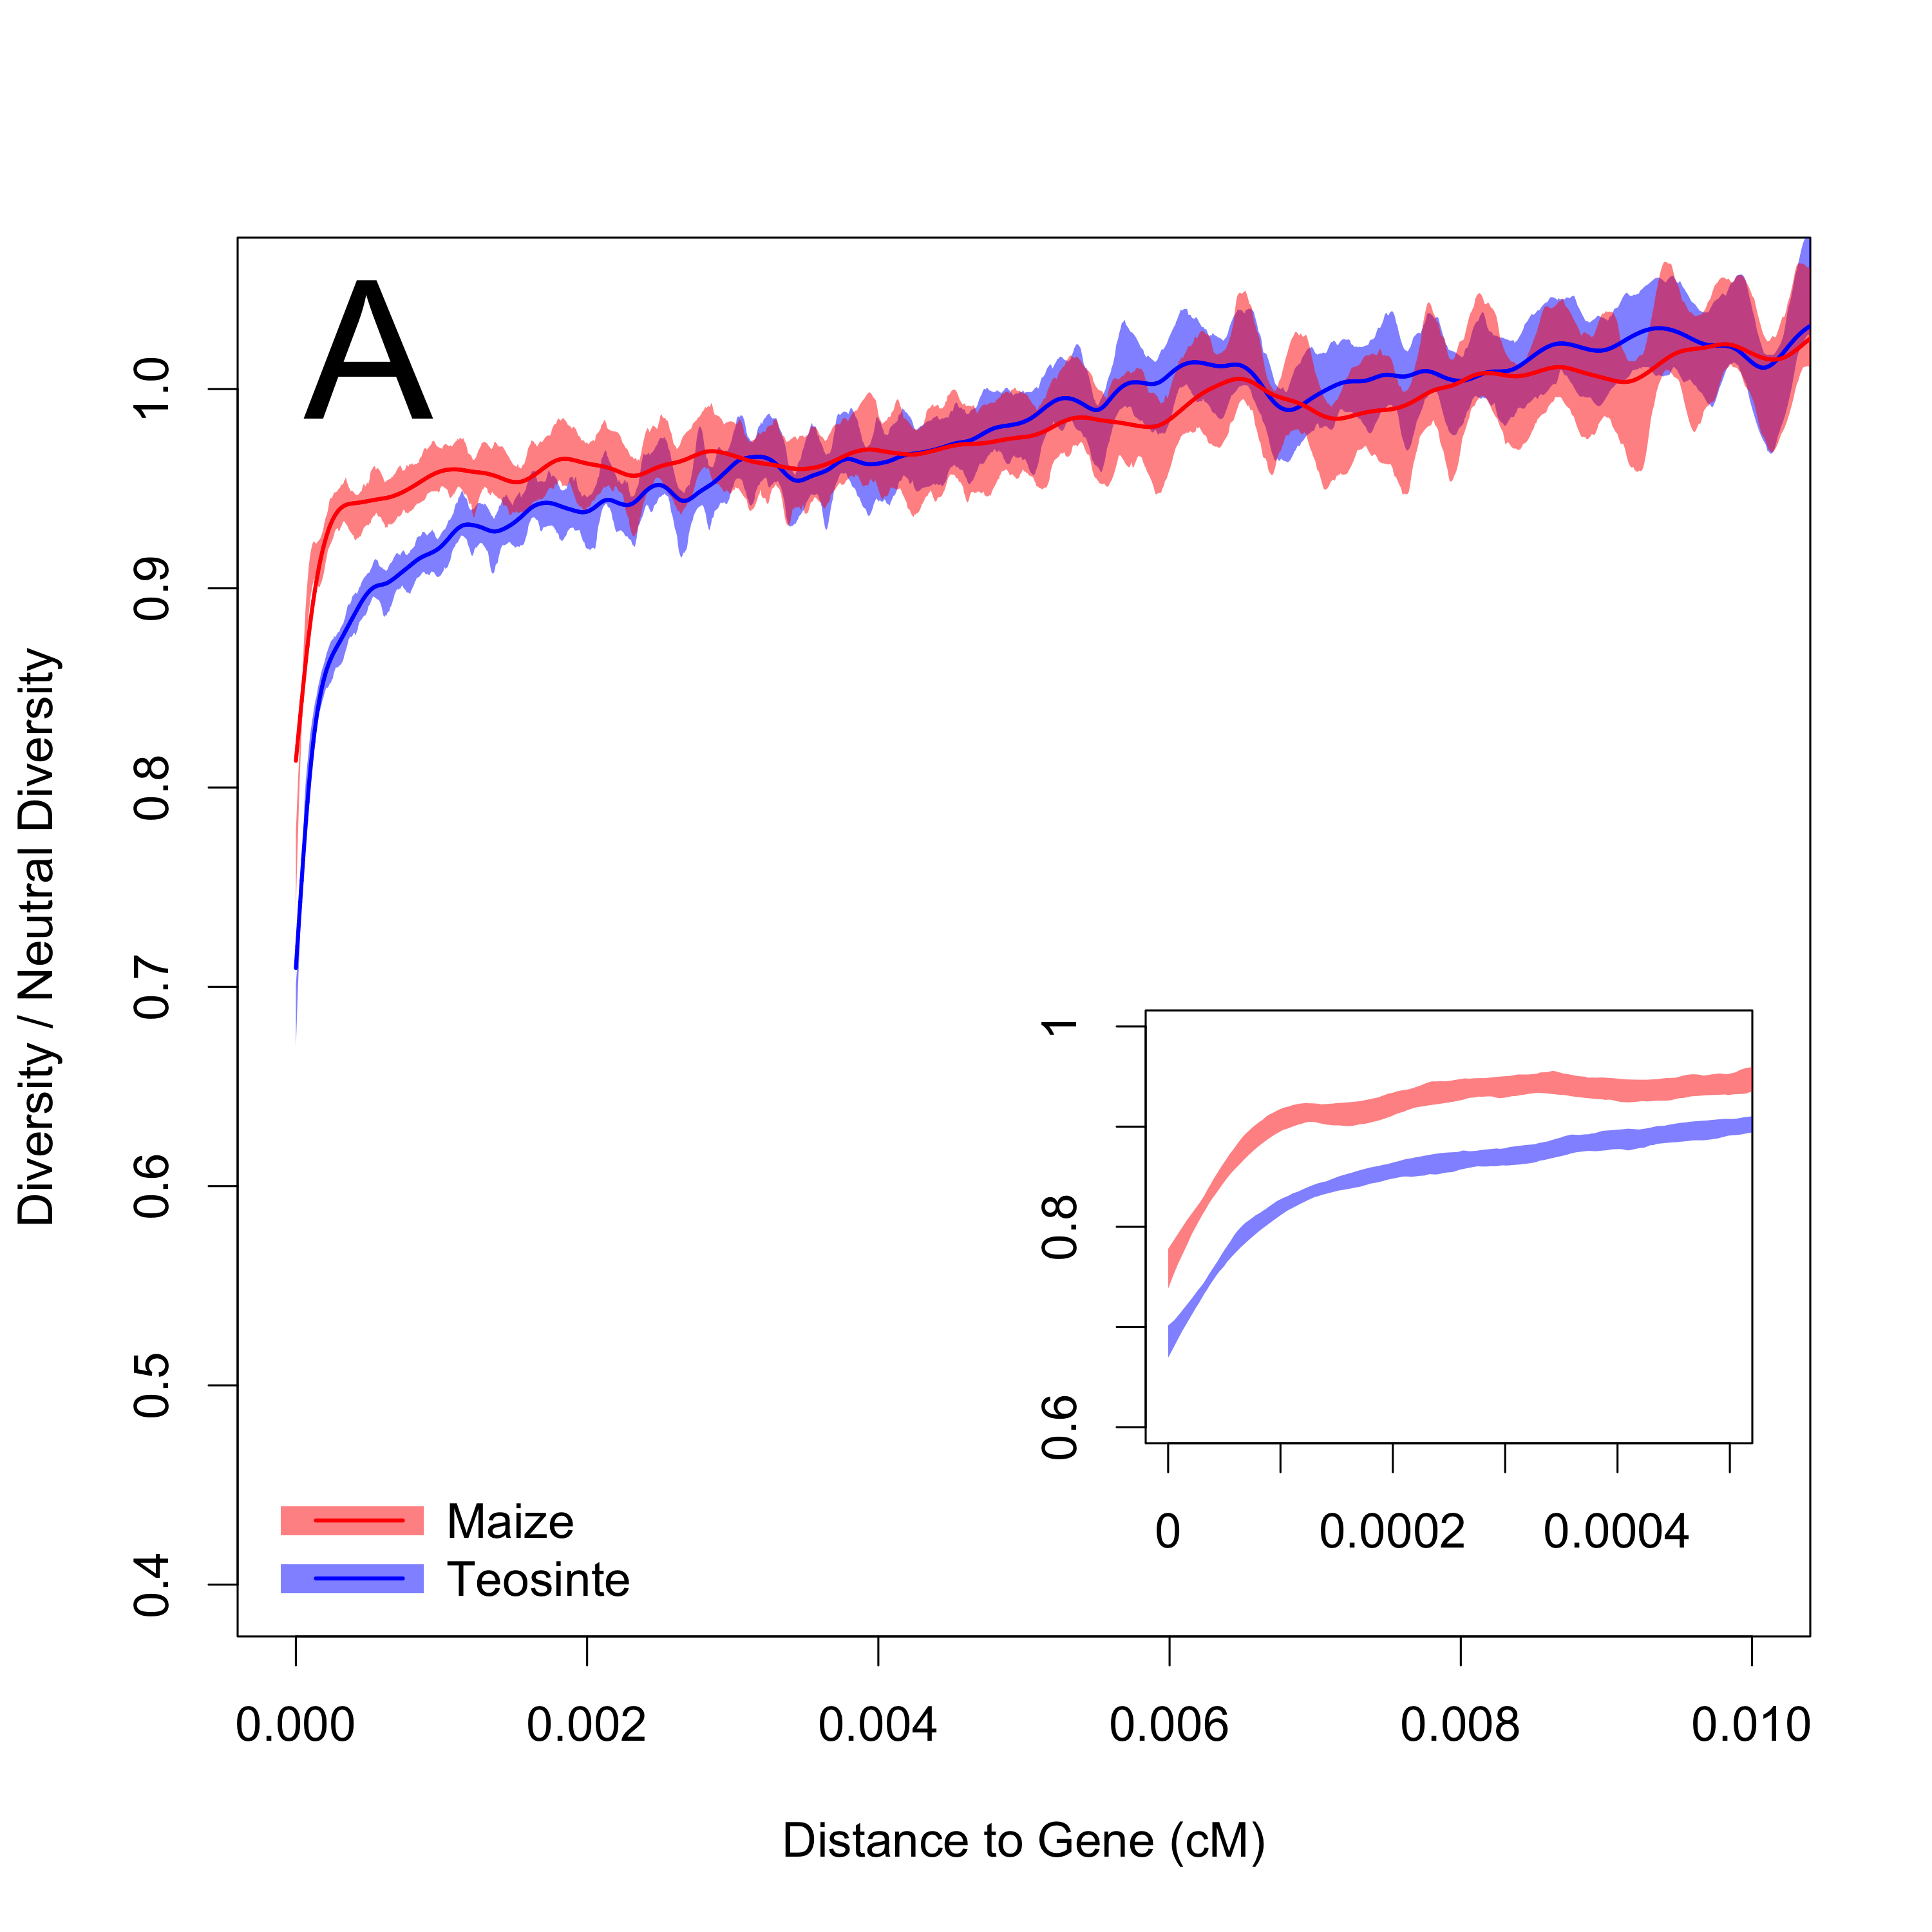
\includegraphics[width=.45\textwidth]{figs/distanceToGene_WithSignificance_Folded2_manuscript.png} 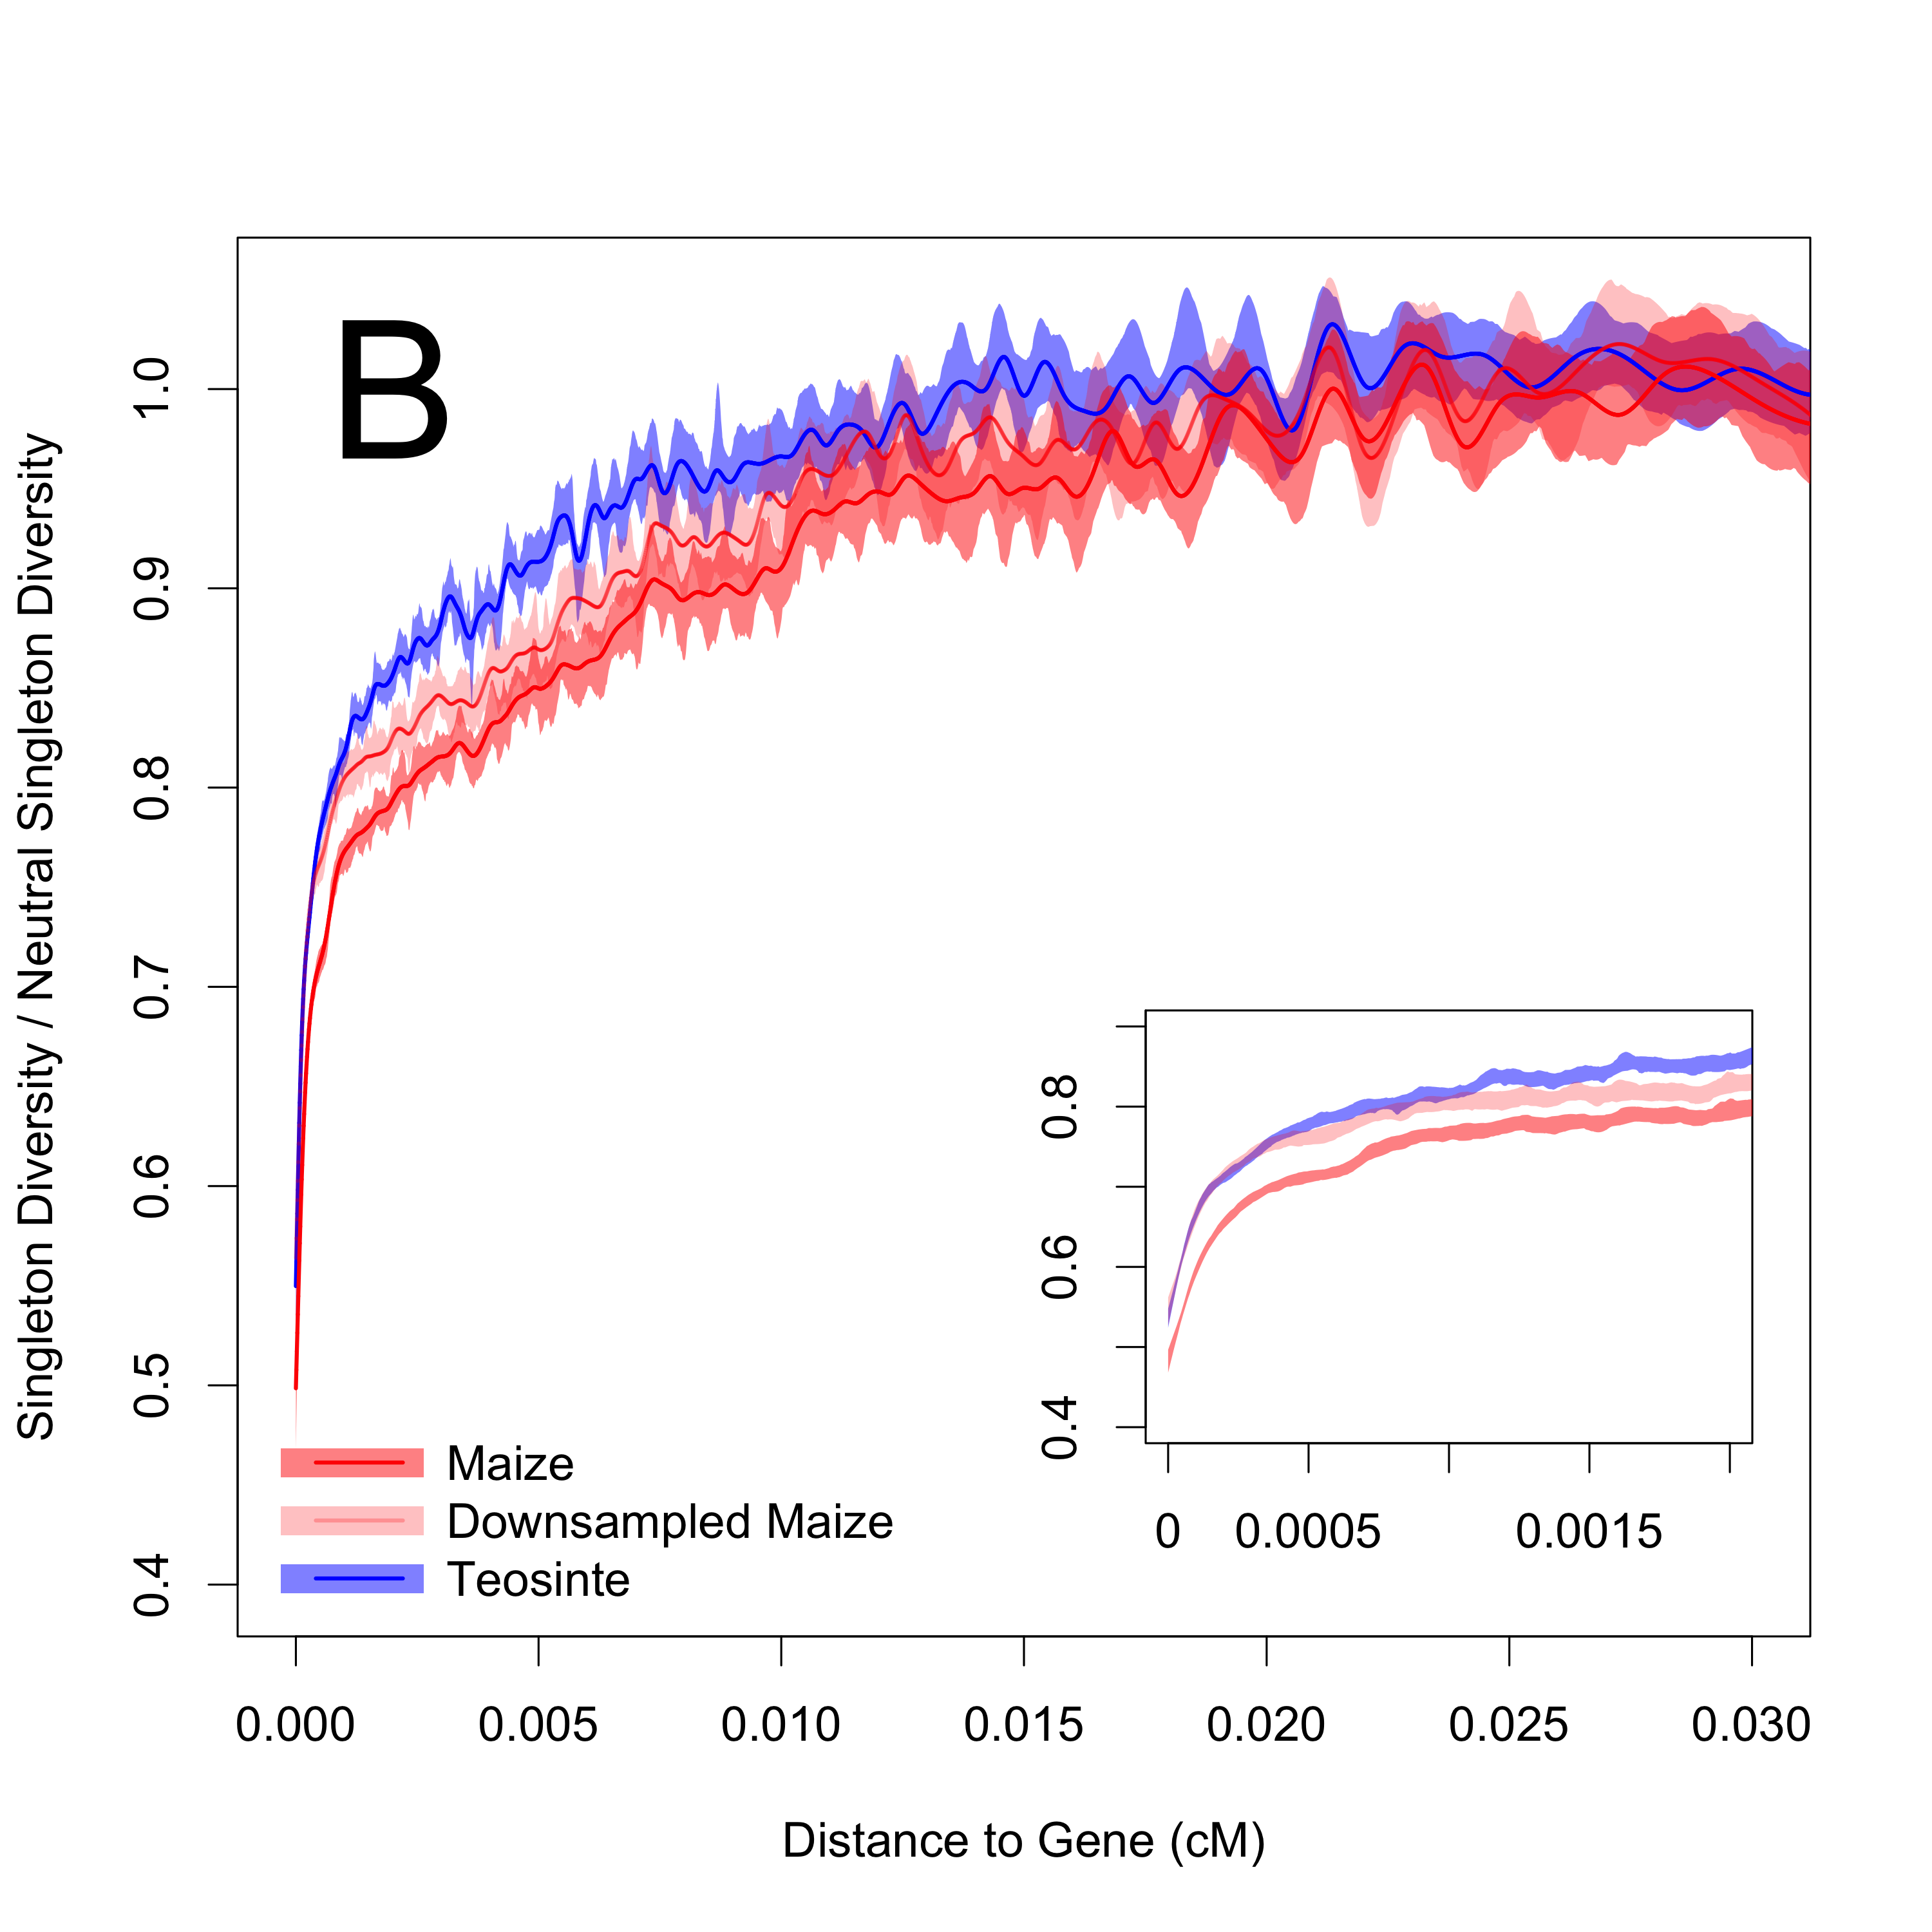
\includegraphics[width=.45\textwidth]{figs/distanceToGene_WithSignificance_Singletons_Downsampled_threeLines_manuscript.png}
\caption{Relative pairwise nucleotide diversity (A) and singleton diversity (B) as a function of distance to the nearest gene.  
\label{fig:purify}}
\end{figure*}

Our current work on domestication focuses on how the processes of demographic change and adaptation have shaped genetic and phenotypic diversity.
Maize underwent a demographic bottleneck during domestication, reducing its effective population size and thus the efficacy of purifying selection.
Indeed, purifying selection in teosinte is stronger due to its larger effective population size, resulting in both a deeper and wider valley of diversity around conserved genes (Figure \ref{fig:purify}A).
But maize population grew quickly after domestication, eventually exceeding that of teosinte.
New mutations in maize are thus subject to stronger selection than in teosinte, a shift reflected in patterns of variation in recent low frequency variants such as singleton polymorphisms (Figure \ref{fig:purify}B).   
Population demographic change can also impact the size, number, and dominance of loci underlying phenotypic traits \citep{lohmueller2014impact,gazave2013population}.
Our future work will utilize data from large-scale association mapping studies, coupled with population genomic inference of demographic change and selection, to study how the process of domestication may have shaped the genetic architecture of phenotypic traits.

Building on our work highlighting the importance of deleterious alleles in phenotypic variation \citep{mezmouk2014pattern}, we have used experimentally evolved populations to track haplotype frequencies over time and assess the genetic basis of gain in hybrid yield. 
Our recent analysis finds little overlap in selected haplotypes between two populations bred for increasing hybrid yield, consistent with a model for complementation of deleterious variants brought to high frequency by hitchhiking  \citep{gerke2013genomic}. 
We are now working to extend these analyses has combined genotype and historical data to build a pedigree of more than 4,000 maize lines with which to extend these haplotype analyses across many populations.  

\section*{Local adaptation} %369
% architecture, biotic interactions, climate, introgression

After domestication, maize spread rapidly, adapting to a wide range of environments. 
Today maize is grown across a broader geographic breadth than any of the world's other staple crops \citep{hake2015genetic}, from sea level to altitudes of $>4,000$m and from deserts to near-flooded conditions.
The wild relatives of maize have also adapted to environments varying widely in elevation, temperature, and moisture gradients. 
Our previous work has shown that adaptation in teosinte is often restricted to discrete local populations and has often made use of regulatory variation \citep{pyhajarvi2013complex}.
We also find evidence that inversion polymorphisms are common and associated with environmental gradients and phenotypic variation \cite{pyhajarvi2013complex,fang2012megabase}.
In contrast to classical expectations of underdominance, even large inversion polymorphisms appear able to circumvent problems of underdominance in heterozygotes without negatively affecting normal chromosomal pairing \citep{maguire1966relationship}.
We suspect such structural variation is common in complex plant genomes, and work is underway both to characterize the genomic and phenotypic effects of individual inversions and to more broadly characterize structural variation within natural populations.

In many instances of local adaptation, independent populations have converged on similar phenotypic adaptations.  
We have worked with maize populations adapted to high elevation environments in Mexico and South America, seeking to understand whether convergent phenotypic evolution is associated with convergent evolution at the molecular level.
Our previous efforts pointed to a key role for adaptive introgression from wild teosinte in enabling maize to adapt to the mountains of central Mexico \citep{hufford2013genomic}, but in spite of similar phenotypes our recent work shows virtually no overlap between Mexican and Andean maize populations in the genes most affected by selection \citep{Takuno15062015}.
Our population genetic analyses suggest that most local adaptation in these populations has not been mutation limited, but that instead stochastic differences in local founding populations, each with abundant standing genetic variation, likely explains the lack of convergent genetics.

Our current work on local adaptation builds on these results, focusing on detailed characterization of individual populations of both maize and teosinte. 
We are making use of deep sequencing of the genome and methylome of a number of individuals, combined  with common garden evaluation of progeny, to identify the loci and processes involved in adaptation at an extremely local scale and ask how these differ from processes operating species-wide.

%{
%\color{red}  
%\noindent\makebox[\linewidth]{\rule{\linewidth}{0.4pt}}
%STOP HERE \\
%\noindent\makebox[\linewidth]{\rule{\linewidth}{0.4pt}}
%}

\section*{Genome evolution} %345

In addition to discerning the genetic basis of phenotypic evolution, we are interested in  understanding the processes that shape evolution of the genome itself.
We have shown that differences in deletion bias can effect large changes in genome size over phylogenetic time scales \citep{tenaillon2011genome}, and documented extensive variation in copy number across diverse maize and teosinte \citep{gore2009first, chia2012maize}.
Current work characterizing copy number variation in a single wild population of teosinte has revealed problems with population genetic methods that assume data is missing due to stochastic sampling.
Tajima's D, for example, shows a strong positive correlation with CNV frequency, potentially leading to misinterpretation of selection or demographic change if biologically missing data was not accounted for.

The single largest component of the maize genome --- and of the majority of flowering plants --- is transposable elements (TEs). 
We have previously shown important functional consequences of individual TE insertions on phenotype and gene expression \cite{studer2011identification,makarevitch2015transposable}, we are just beginning to understand their genome-wide significance.
We have recently re-annotated all of the retroelements in the maize genome ($>70\%$ of the genome), and are now using high-throughput sequencing and our annotation to identify new insertions in nonreference genomes. 
Analysis of the first deeply sequenced inbred, for example, revealed 350,000 high-confidence nonreference insertions, of which nearly 3,000 were into CDs of annotated genes.
We are currently evaluating the impacts of these insertions on patterns of methylation and gene expression across a panel of inbred lines, and in the future will apply these methods to natural populations.

\begin{figure*}[]
\centering
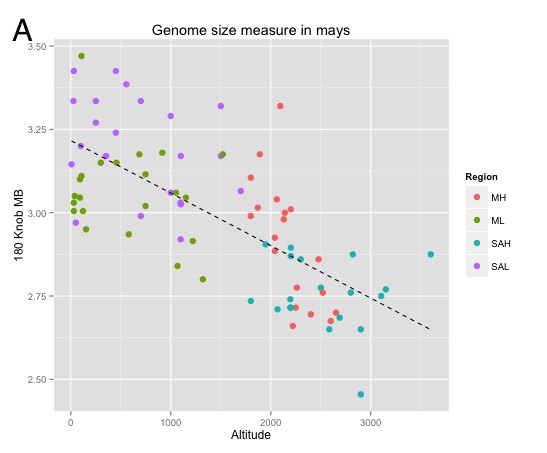
\includegraphics[width=.45\textwidth]{figs/gsjeff} 
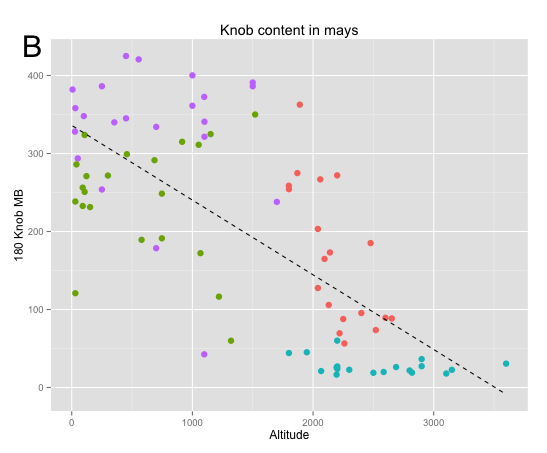
\includegraphics[width=.45\textwidth]{figs/knobjeff}
\caption{Heterochromatic knob abundance (A) and 1C genome size (B) as a function of elevation. Data are shown from Mexican (M) and South American (SA) highland (H) and lowland (L) populations.
\label{fig:gsize}}
\end{figure*}

Finally, in one project underway we are modeling the genome as a phenotype to understand the evolutionary processes shaping genome size change.
Building on prior observations of genome size variation, we have developed methods to quantify the abundance of repetitive fractions of the genome and test for selection on repeat abundance after controlling for relatedness. 
We find that both overall genome size (Figure \ref{fig:gsize}A) and, in spite of their potential for meiotic drive, heterochromatic knob abundance (Figure \ref{fig:gsize}B) both show evidence of selection for smaller genomes across altitudinal gradients, perhaps as a means of accelerating development and flowering.

%
%\begin{figure*}[tb]
%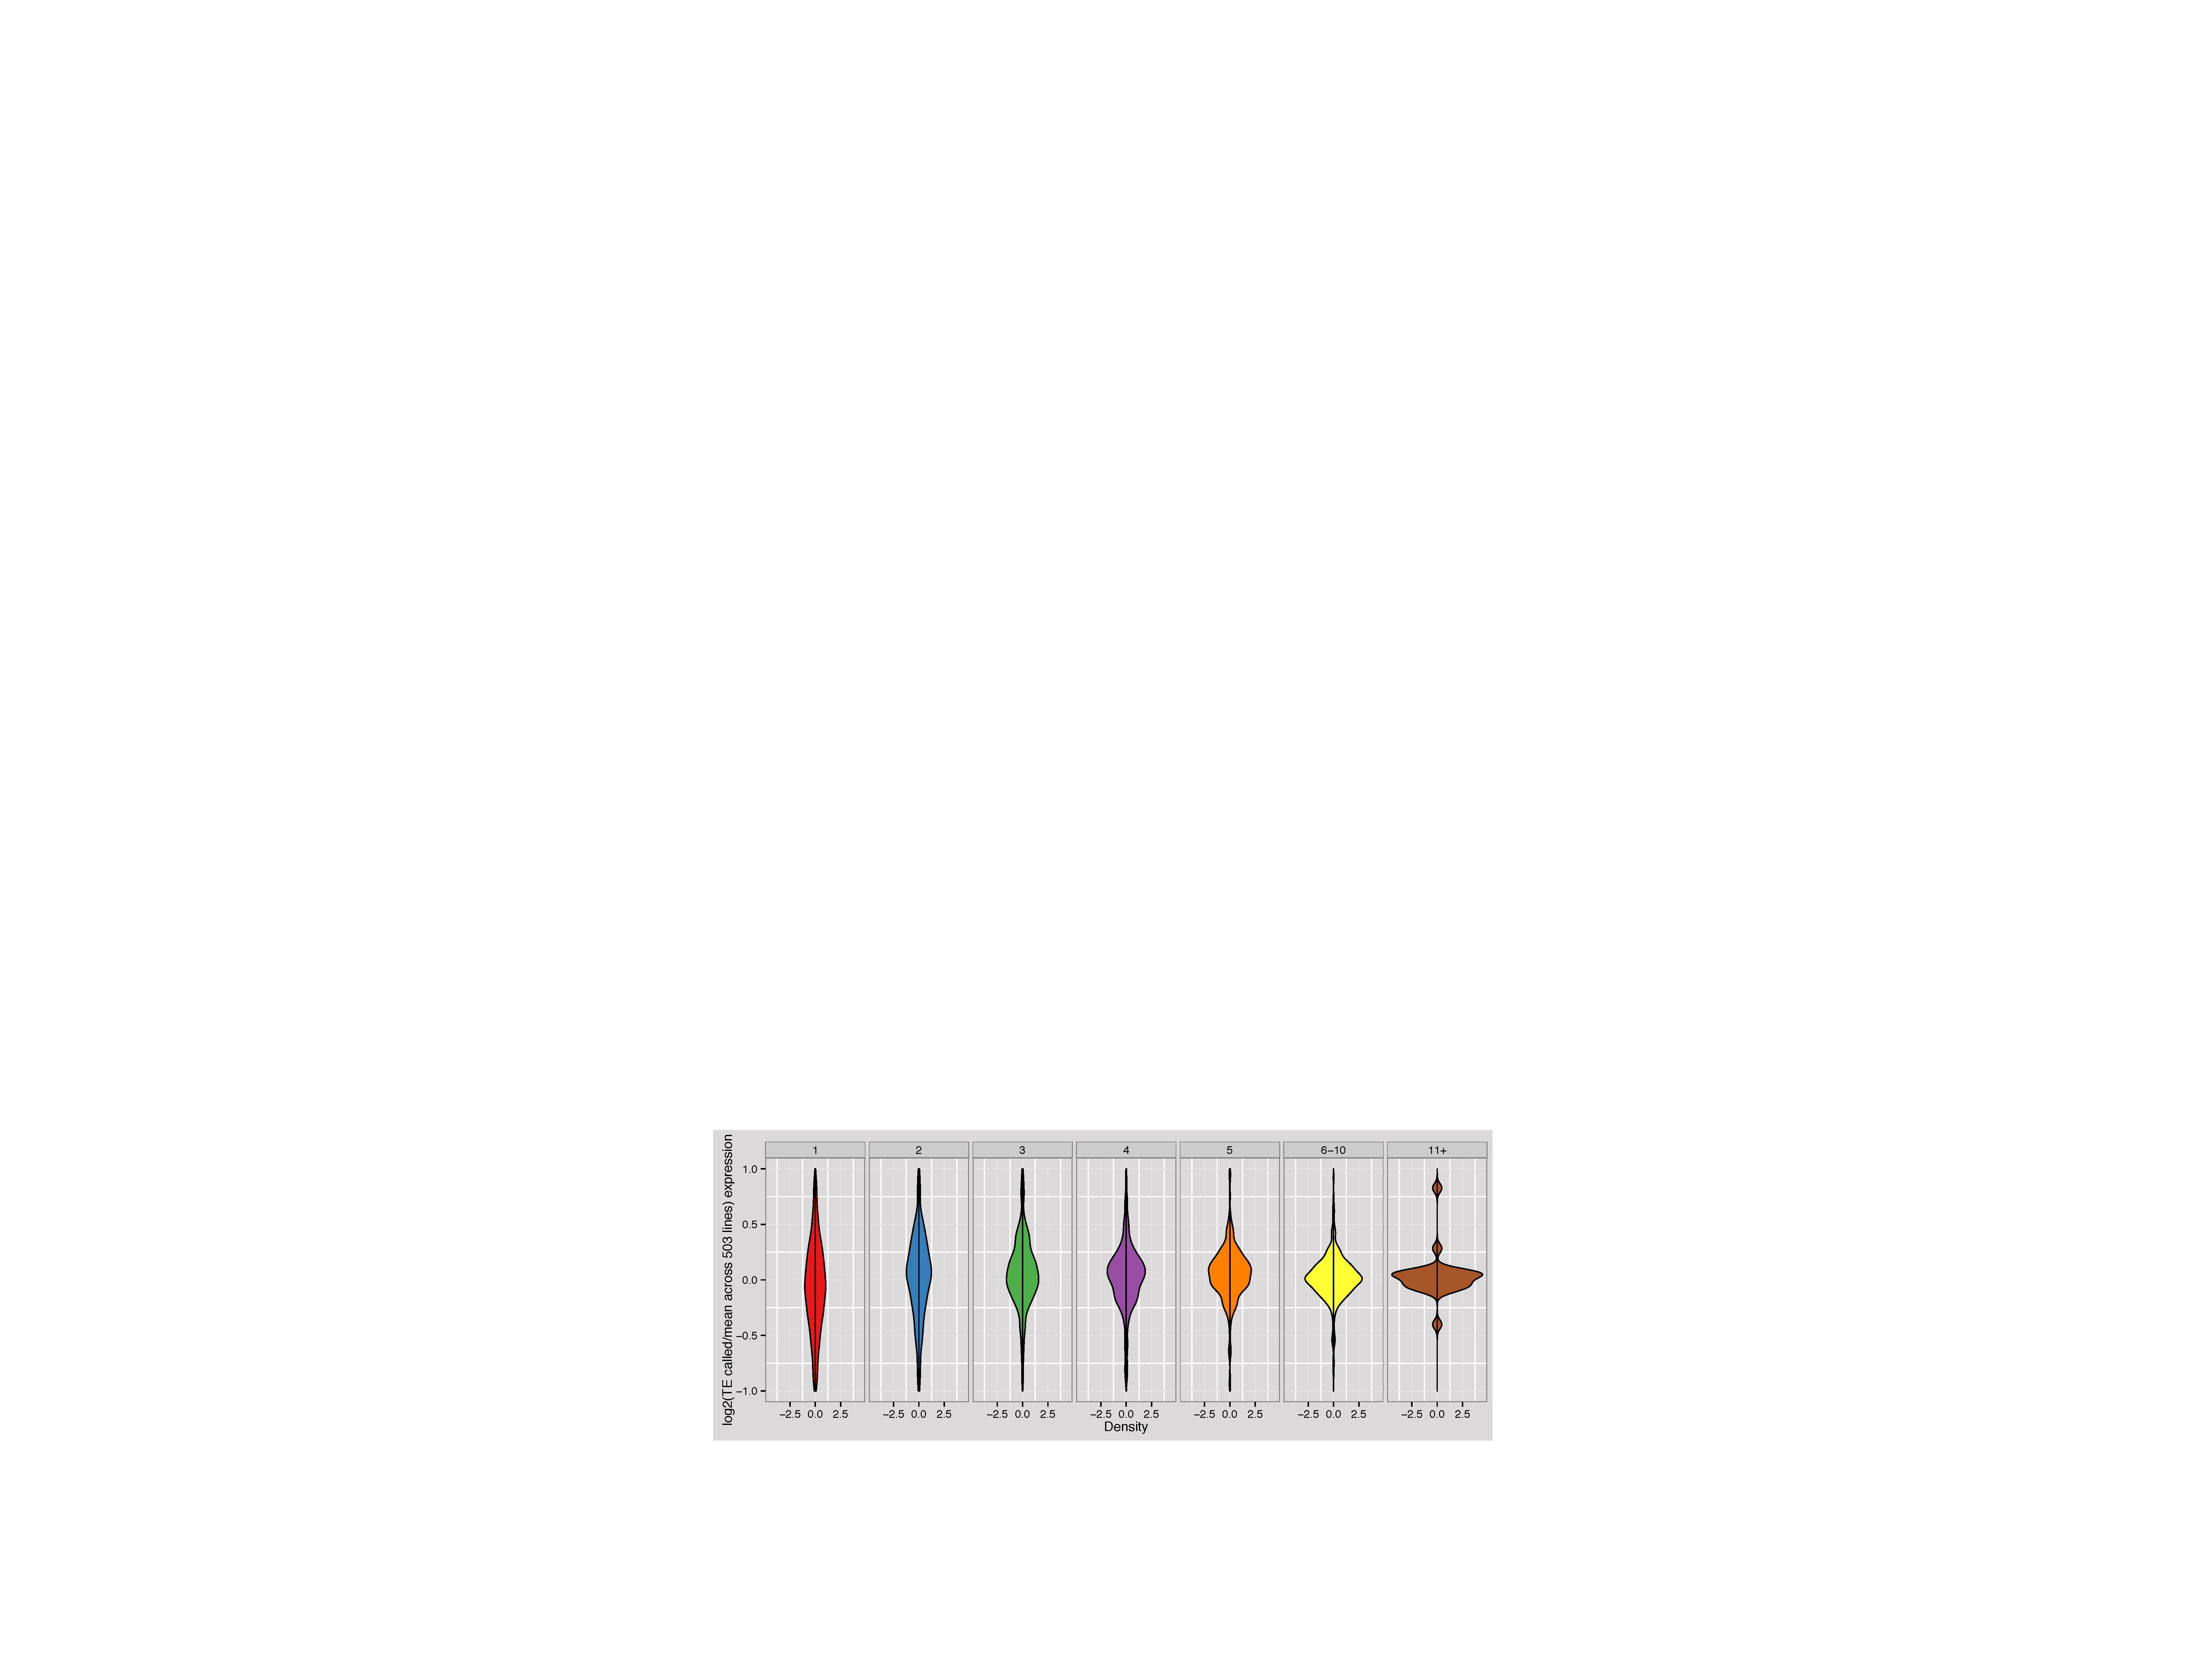
\includegraphics[width=0.45\linewidth]{figs/te_expression.pdf}
%\caption{The effect of \emph{de novo} non-reference transposable element insertion on gene expression. Panels show the impact of insertions identified in 1 (far left) to $>10$ (far right) inbred lines in a panel of 23 maize inbreds.  Shown in each panel is the relative expression of genes in inbred lines with the insertion within the annotated gene region to the mean expression of that gene across 500 maize lines \citep{hirsch2014insights}. Recent, low frequency insertions tend to decrease gene expression compared to older, high-frequency insertions.  } 
%\label{fig:te_expression}
%\end{figure*}
%
%\begin{SCfigure}
%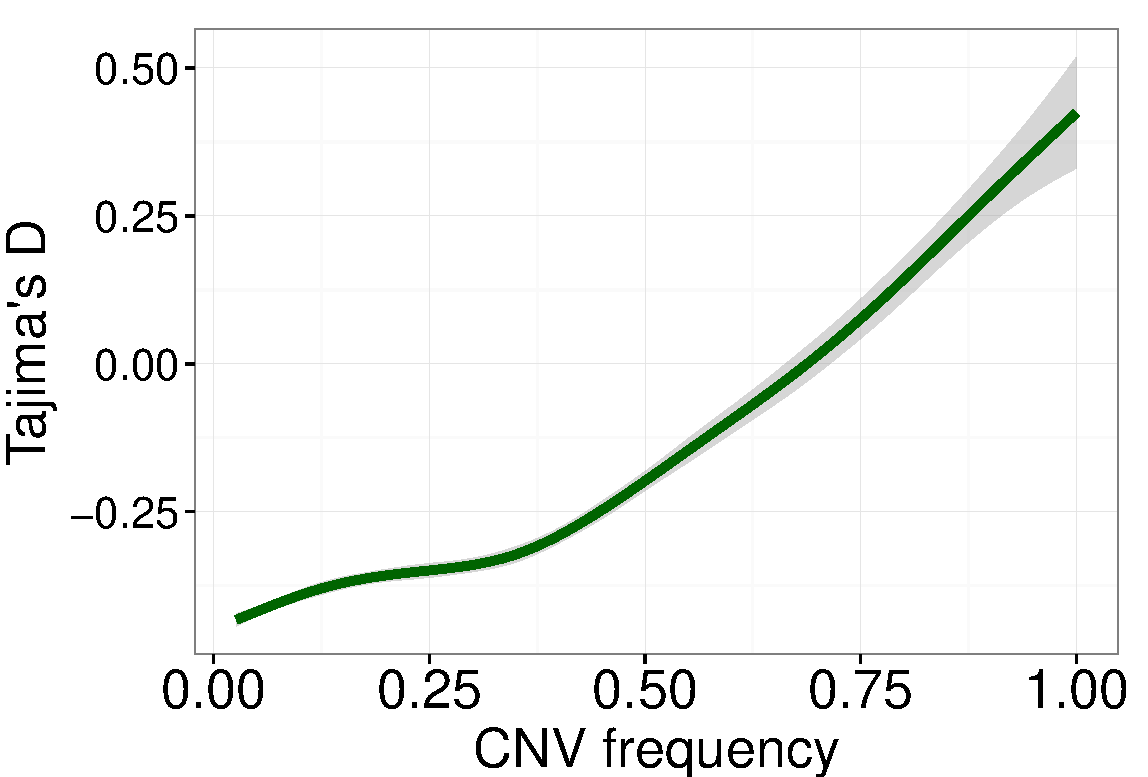
\includegraphics[width=0.3\linewidth]{figs/td_cnv.pdf}
%\caption{The effect of copy number variation (CNV) on estimates of Tajima's D, a measure of the allele freqeuncy spectrum. In regions with no CNV, Tajima's D is negative consistent with population expansion. Tajima's D is inferred to be strongly postiive in regions with high-frequency CNVs, however, which could be (erroneously) interpreted as population decline or balancing selection.} 
%\label{fig:tajd}
%\end{SCfigure}
%

%\section*{Notes}
%
%\citep{peischl2015expansion} predict more u-shaped SFS in expanded pops, also more homozygous deleterious. this is seen in humans. Li's results in maize
%
%\citep{fu2014characteristics}
%``Indeed, a substantial amount of the higher density of deleterious alleles in EA individuals in the simulated data is attributable to weakly deleterious mutations $(|s| \approx 10^{-4})$''
%
%\citep{balick2013response} show weighted sum of the SFS can be used to differentiate recessive vs. not at deeteirous sites.
%
%\citep{lohmueller2014impact} 
%``Under a model where a mutation's effect on a trait is correlated with its effect on fitness, rare variants explain a greater portion of the additive genetic variance of the trait in a population that has recently expanded than in a population that did not recently expand. Further, when using a single-marker test, for a given false-positive rate and sample size, recent population growth decreases the expected number of significant associations with the trait relative to the number detected in a population that did not expand. However, in a model where there is no correlation between a mutation's effect on fitness and the effect on the trait, common variants account for much of the additive genetic variance, regardless of demography.''
%
%\citep{tennessen2012evolution} Shows vast majority of functionally important alleles rare, attributes to explosive population growth and weak purifying selection
%
%\citep{hufford2013genomic} \citep{hufford2012comparative}

\newpage
\bibliography{jri.bib}
\end{document}
